\section*{Глава 2. Проектирование веб-приложения}
\addcontentsline{toc}{section}{Глава 2. Проектирование веб-приложения}
\stepcounter{section}

\subsection{Анализ целевой аудитории}

Разрабатываемая платформа ориентирована на людей, изучающих английский язык
и заинтересованных в разговорной практике в групповом формате. Основное ядро
аудитории составляют студенты и работающие специалисты в возрасте 18--35 лет,
владеющие языком на уровне A2--C1 по шкале CEFR и испытывающие потребность
в регулярной устной практике с живыми собеседниками. К второстепенным сегментам
относятся преподаватели-энтузиасты, ведущие разговорные клубы, и администраторы
учебных заведений, организующие внеучебные мероприятия.

Ключевая проблема, которую решает платформа, -- разрозненность информации
о разговорных клубах: расписания публикуются в социальных сетях, мессенджерах
и сообществах вузов, что затрудняет поиск встречи подходящего уровня
в удобное время. Существующие альтернативы (Meetup, Telegram-каналы)
не учитывают уровень языка участников и не предоставляют единого каталога.

В системе выделяются три роли пользователей.

\textbf{Участник} -- любой зарегистрированный пользователь. Ведёт профиль
с уровнем языка (CEFR), просматривает каталог клубов, записывается на встречи.
Может в любой момент создать клуб, став его организатором.

\textbf{Организатор} -- пользователь, создавший один или несколько клубов.
Управляет расписанием встреч, просматривает список записавшихся участников
и выгружает его в CSV для подготовки к занятию.

\textbf{Администратор} -- привилегированный пользователь, ответственный за
модерацию платформы. Блокирует нарушителей, скрывает неактивные клубы
и имеет доступ ко всем данным системы.

Для каждой роли составлен профиль пользователя (Persona), отражающий типичный
сценарий использования платформы (таблица~\ref{tab:personas}).

\begin{table}[h]
\centering
\caption{Профили пользователей (Personas)}
\label{tab:personas}
\begin{tabular}{|p{3.5cm}|p{4.5cm}|p{5.6cm}|}
\hline
\textbf{Роль} & \textbf{Цель} & \textbf{Типичное действие} \\
\hline
Участник & Найти встречу своего уровня и записаться &
Открыть каталог, выставить фильтр по уровню CEFR,
выбрать встречу, нажать «Записаться» \\
\hline
Организатор & Набрать группу и провести встречу &
Создать клуб, добавить встречу, скачать CSV
со списком участников \\
\hline
Администратор & Поддерживать качество контента &
Просмотреть жалобы, заблокировать нарушителя,
скрыть неактивный клуб \\
\hline
\end{tabular}
\end{table}

\subsection{Описание функциональности приложения}

Функциональные возможности системы определяются через взаимодействие
пользователей трёх ролей с платформой. Участник просматривает каталог клубов,
фильтрует встречи по уровню языка и дате, записывается на встречи и управляет
своим профилем. Организатор, являясь участником, дополнительно создаёт клубы
и встречи, отслеживает наполнение группы и выгружает список участников
в CSV-файл. Администратор модерирует пользователей и клубы платформы.

На рисунке~\ref{fig:usecase} представлена диаграмма вариантов использования
системы.

\begin{figure}[h]
\centering
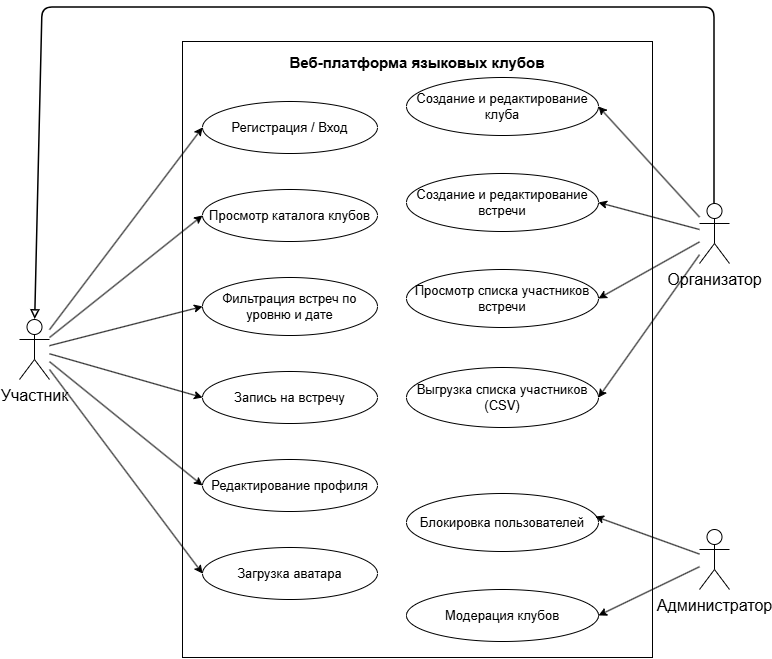
\includegraphics[width=\textwidth]{images/usecase}
\caption{Диаграмма вариантов использования системы}
\label{fig:usecase}
\end{figure}

\clearpage

\subsection{Проектирование модели данных}

На рисунке~\ref{fig:er} представлена ER-диаграмма базы данных.

\begin{figure}[h]
\centering
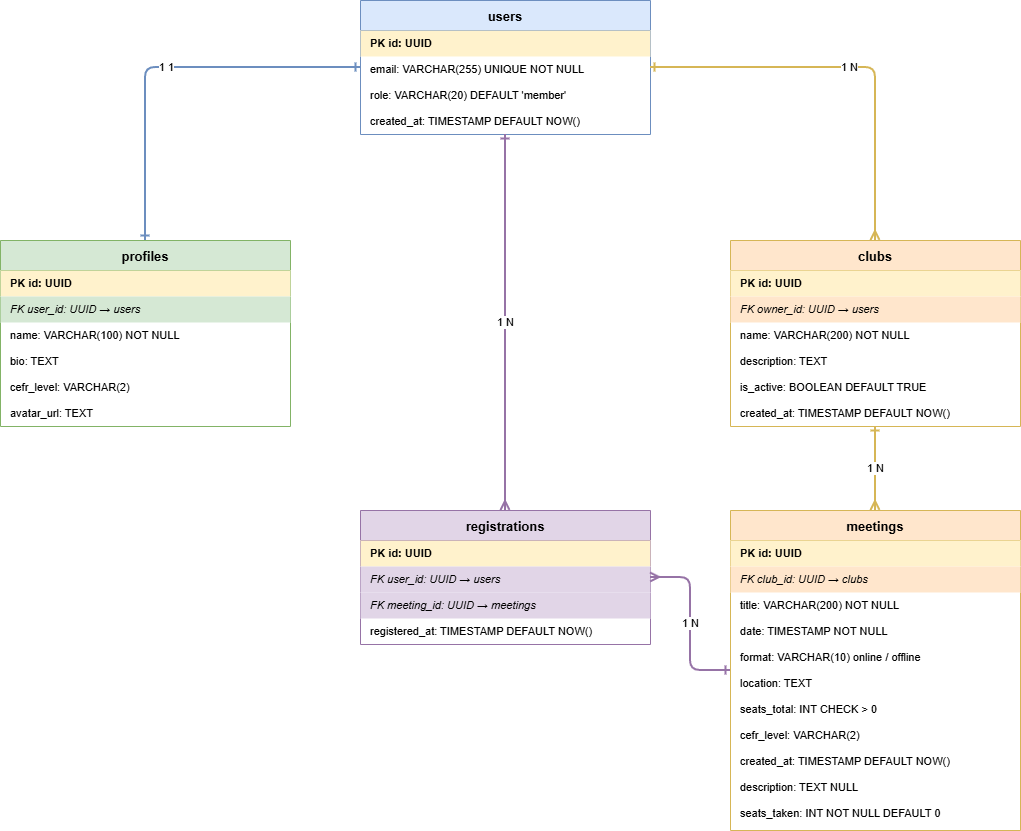
\includegraphics[width=\textwidth]{images/er}
\caption{ER-диаграмма базы данных}
\label{fig:er}
\end{figure}

База данных реализована на PostgreSQL в составе платформы Supabase. Логическая
схема включает пять таблиц, структура которых представлена ниже.

\begin{table}[h]
\centering
\caption{Структура таблицы users (управляется Supabase Auth)}
\label{tab:users}
\begin{tabular}{|p{3cm}|p{3.5cm}|p{3.5cm}|p{3.5cm}|}
\hline
\textbf{Поле} & \textbf{Тип} & \textbf{Ограничение} & \textbf{Описание} \\
\hline
id & UUID & PRIMARY KEY & Уникальный идентификатор \\
\hline
email & VARCHAR(255) & UNIQUE, NOT NULL & Адрес электронной почты \\
\hline
created\_at & TIMESTAMP & DEFAULT NOW() & Дата регистрации \\
\hline
\end{tabular}
\end{table}

\begin{table}[h]
\centering
\caption{Структура таблицы profiles}
\label{tab:profiles}
\begin{tabular}{|p{3cm}|p{3.5cm}|p{3.5cm}|p{3.5cm}|}
\hline
\textbf{Поле} & \textbf{Тип} & \textbf{Ограничение} & \textbf{Описание} \\
\hline
id & UUID & PRIMARY KEY & Уникальный идентификатор \\
\hline
user\_id & UUID & FOREIGN KEY & Ссылка на таблицу users \\
\hline
name & VARCHAR(100) & NOT NULL & Отображаемое имя \\
\hline
bio & TEXT & NULL & Описание <<о себе>> \\
\hline
cefr\_level & VARCHAR(2) & NULL & Уровень языка: A1--C2 \\
\hline
avatar\_url & TEXT & NULL & URL аватара в хранилище \\
\hline
role & VARCHAR(20) & DEFAULT 'member' & Роль: member / admin \\
\hline
\end{tabular}
\end{table}

\begin{table}[h]
\centering
\caption{Структура таблицы clubs}
\label{tab:clubs}
\begin{tabular}{|p{3cm}|p{3.5cm}|p{3.5cm}|p{3.5cm}|}
\hline
\textbf{Поле} & \textbf{Тип} & \textbf{Ограничение} & \textbf{Описание} \\
\hline
id & UUID & PRIMARY KEY & Уникальный идентификатор \\
\hline
owner\_id & UUID & FOREIGN KEY & Создатель клуба (ссылка на users) \\
\hline
name & VARCHAR(200) & NOT NULL & Название клуба \\
\hline
description & TEXT & NULL & Описание клуба \\
\hline
is\_active & BOOLEAN & DEFAULT TRUE & Признак активности \\
\hline
created\_at & TIMESTAMP & DEFAULT NOW() & Дата создания \\
\hline
\end{tabular}
\end{table}

\clearpage

\begin{table}[h]
\centering
\caption{Структура таблицы meetings}
\label{tab:meetings}
\begin{tabular}{|p{3cm}|p{3.5cm}|p{3.5cm}|p{3.5cm}|}
\hline
\textbf{Поле} & \textbf{Тип} & \textbf{Ограничение} & \textbf{Описание} \\
\hline
id & UUID & PRIMARY KEY & Уникальный идентификатор \\
\hline
club\_id & UUID & FOREIGN KEY & Клуб встречи (ссылка на clubs) \\
\hline
title & VARCHAR(200) & NOT NULL & Тема встречи \\
\hline
description & TEXT & NULL & Описание встречи \\
\hline
date & TIMESTAMP & NOT NULL & Дата и время начала \\
\hline
location & TEXT & NULL & Адрес проведения \\
\hline
seats\_total & INT & CHECK > 0 & Максимальное число мест \\
\hline
seats\_taken & INT & DEFAULT 0 & Текущее число занятых мест \\
\hline
cefr\_level & VARCHAR(2) & NULL & Целевой уровень участников \\
\hline
created\_at & TIMESTAMP & DEFAULT NOW() & Дата создания записи \\
\hline
\end{tabular}
\end{table}

\begin{table}[h]
\centering
\caption{Структура таблицы registrations}
\label{tab:registrations}
\begin{tabular}{|p{3cm}|p{3.5cm}|p{3.5cm}|p{3.5cm}|}
\hline
\textbf{Поле} & \textbf{Тип} & \textbf{Ограничение} & \textbf{Описание} \\
\hline
id & UUID & PRIMARY KEY & Уникальный идентификатор \\
\hline
user\_id & UUID & FOREIGN KEY & Участник (ссылка на users) \\
\hline
meeting\_id & UUID & FOREIGN KEY & Встреча (ссылка на meetings) \\
\hline
registered\_at & TIMESTAMP & DEFAULT NOW() & Дата и время записи \\
\hline
\end{tabular}
\end{table}

Уникальное ограничение \texttt{UNIQUE(user\_id, meeting\_id)} предотвращает
повторную запись одного участника на ту же встречу.

Счётчик занятых мест \texttt{seats\_taken} в таблице \texttt{meetings} хранится
в денормализованном виде и поддерживается в актуальном состоянии триггерами
\texttt{AFTER INSERT}~/~\texttt{AFTER DELETE} на таблице \texttt{registrations}.
Такой подход выбран по двум причинам. Во-первых, при вычислении счётчика
агрегатным запросом \texttt{COUNT(*)} политика безопасности на уровне строк
(RLS) скрывает чужие записи от пользователя, что приводит к занижению значения.
Во-вторых, отдельная колонка позволяет атомарно проверять наличие свободных
мест в триггере \texttt{BEFORE INSERT}, исключая ситуацию превышения вместимости
при одновременных запросах от нескольких пользователей.

\subsection{Разработка макетов страниц}

Для ключевых страниц разработаны wireframe-макеты, отражающие расположение
функциональных элементов интерфейса.

\textbf{Каталог встреч (рисунок~\ref{fig:wire_catalog})} -- главная страница
платформы. Содержит панель фильтрации по уровню CEFR и диапазону дат, а также
сетку карточек встреч. Каждая карточка отображает тему встречи, дату и время,
адрес, клуб-организатор, уровень языка и счётчик занятых мест.

\begin{figure}[h]
\centering
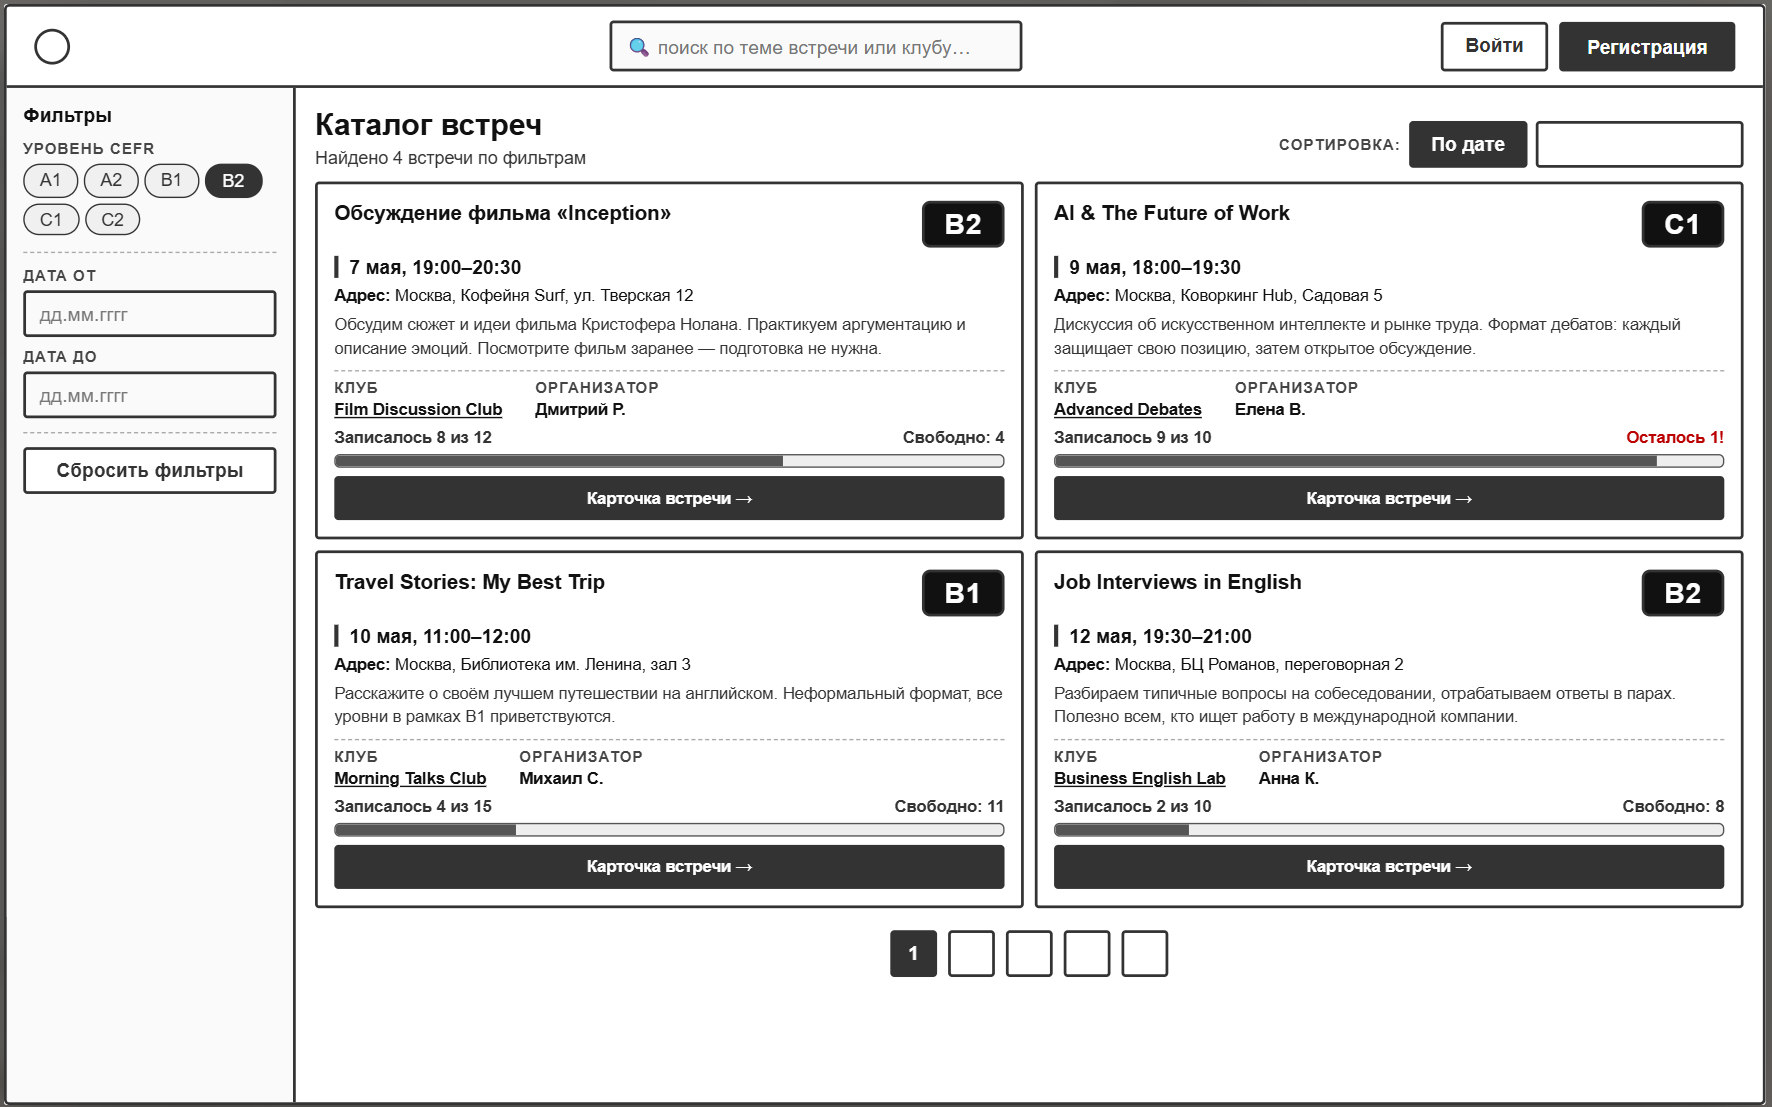
\includegraphics[width=\textwidth]{images/wire_catalog}
\caption{Макет страницы каталога встреч}
\label{fig:wire_catalog}
\end{figure}

\clearpage

\textbf{Карточка встречи (рисунок~\ref{fig:wire_meeting})} -- детальная
страница отдельной встречи. Отображает тему, дату, адрес, клуб, организатора,
описание и уровень языка. В правой части расположен блок записи со счётчиком
<<X из N мест занято>> и кнопкой <<Записаться>>; для уже записавшихся участников
кнопка меняется на <<Отменить запись>>.

\begin{figure}[h]
\centering
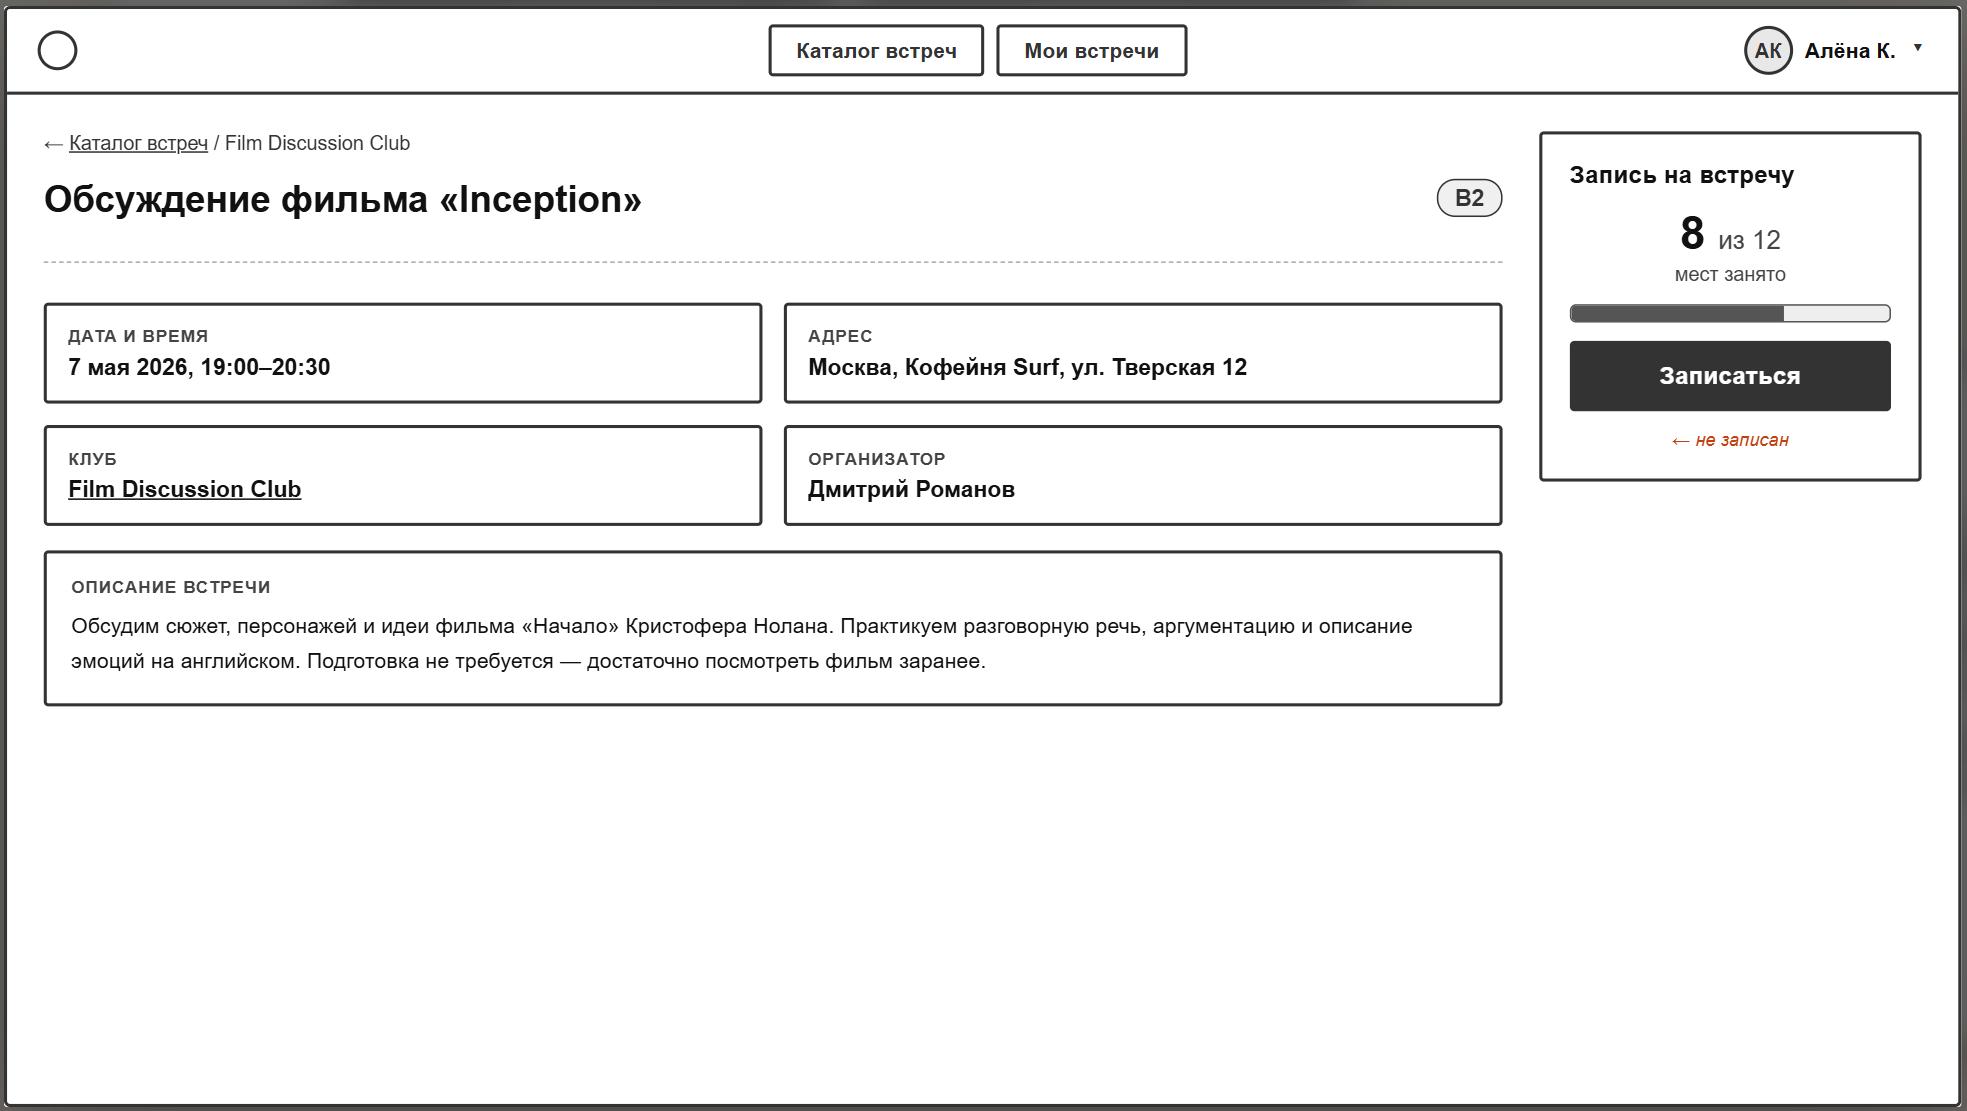
\includegraphics[width=\textwidth]{images/wire_meeting}
\caption{Макет страницы карточки встречи}
\label{fig:wire_meeting}
\end{figure}

\textbf{Профиль участника (рисунок~\ref{fig:wire_profile})} -- личная страница
пользователя. В левой колонке -- аватар, имя, бейдж уровня CEFR и раздел
<<о себе>>. В правой колонке -- форма редактирования профиля с загрузкой
аватара, полями имени и био, выбором уровня языка.

\begin{figure}[h]
\centering
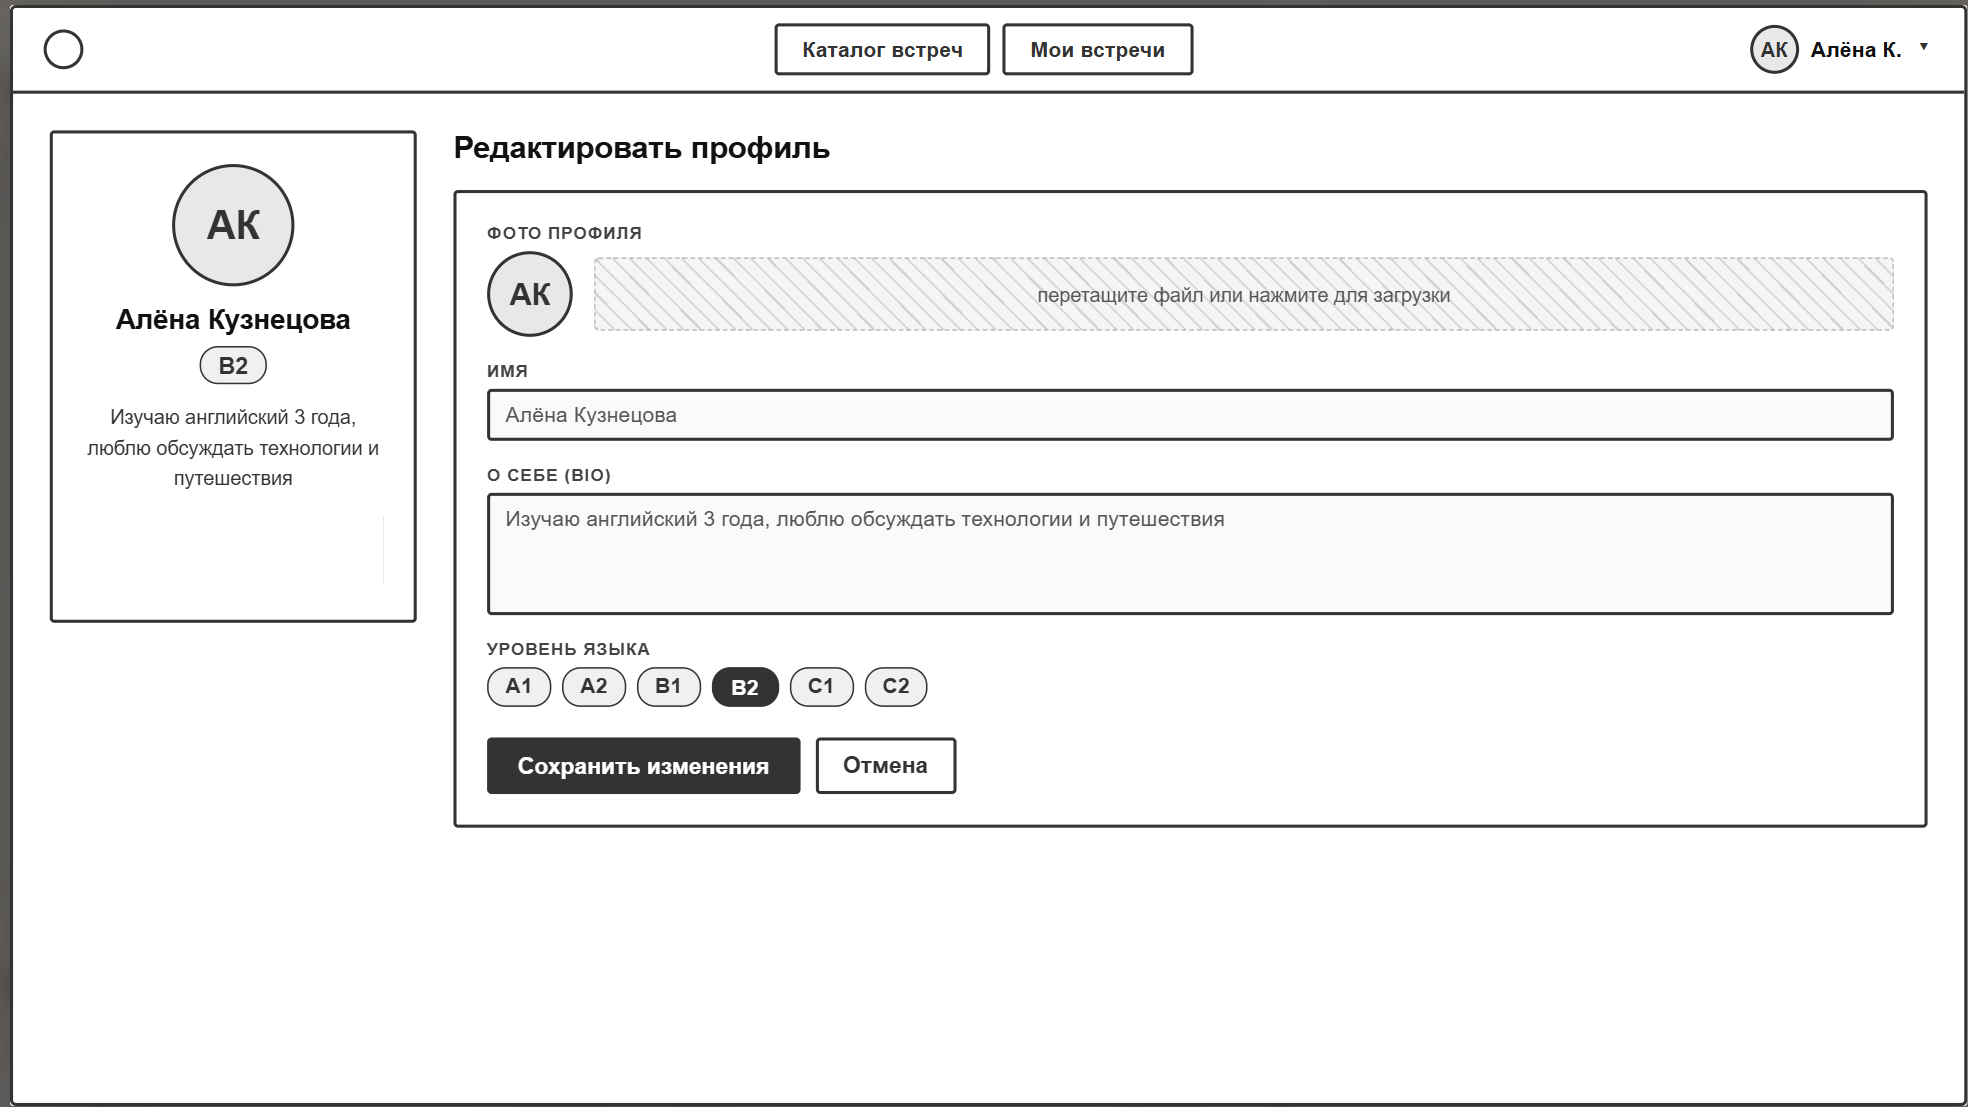
\includegraphics[width=\textwidth]{images/wire_profile}
\caption{Макет страницы профиля участника}
\label{fig:wire_profile}
\end{figure}

\clearpage

\textbf{Панель организатора (рисунок~\ref{fig:wire_organizer})} -- страница
управления клубом. Содержит название и описание клуба, фильтр встреч
(все~/~предстоящие~/~прошедшие), список встреч с прогресс-баром заполненности
и кнопками <<Редактировать>>, <<Удалить>>, <<Скачать CSV>>, а также кнопку
создания новой встречи.

\begin{figure}[h]
\centering
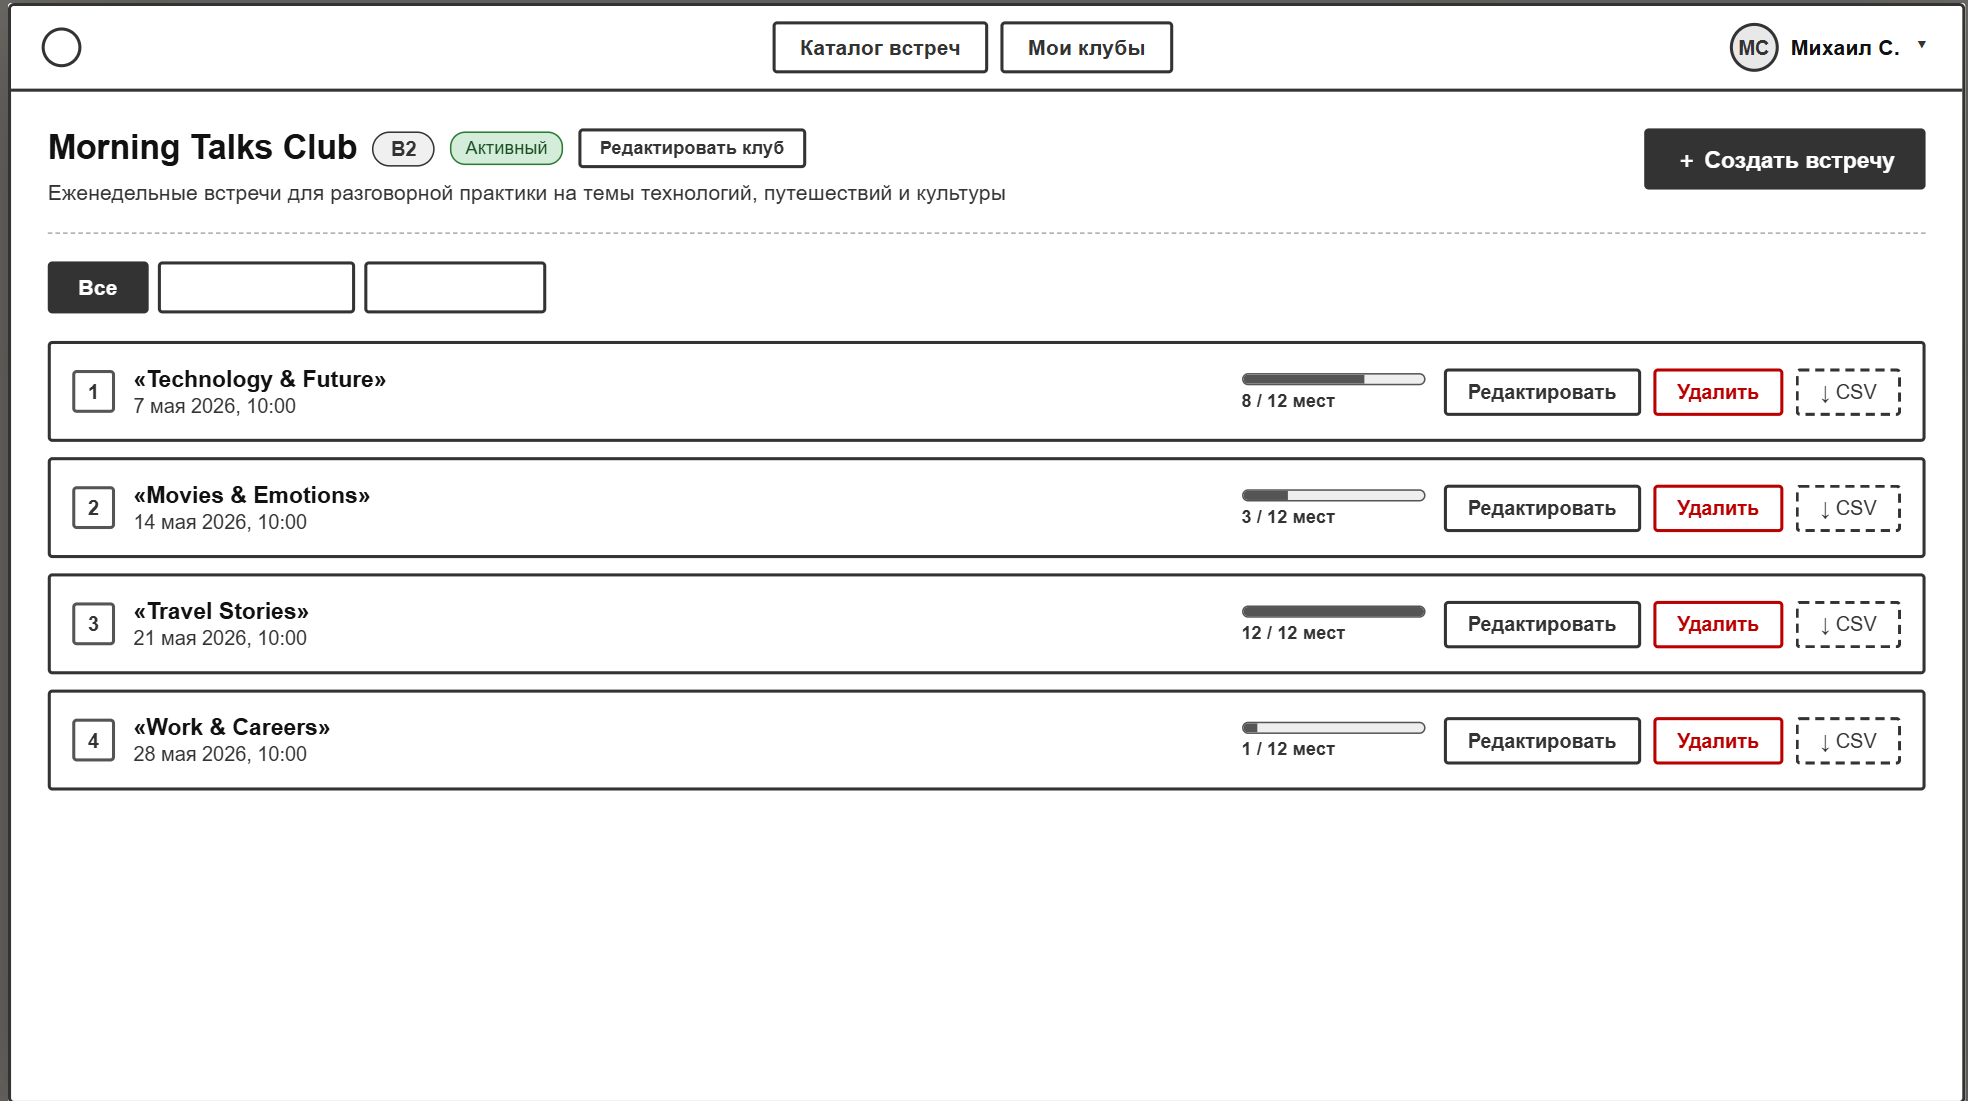
\includegraphics[width=\textwidth]{images/wire_organizer}
\caption{Макет панели организатора}
\label{fig:wire_organizer}
\end{figure}
